\documentclass[border=0.125cm]{standalone}
\usepackage{tikz}
\usetikzlibrary{positioning}
\usetikzlibrary{arrows}
\usetikzlibrary{backgrounds}
\begin{document}

\definecolor{klight_green_200}{RGB}{197, 225, 165}
\definecolor{klight_green_300}{RGB}{174, 213, 129}
\definecolor{klight_green_400}{RGB}{156, 204, 101}
\definecolor{klight_green_500}{RGB}{139, 195, 74}
\definecolor{kgreen_300}{RGB}{129, 199, 132}
\definecolor{kgreen_500}{RGB}{76, 175, 80}
\definecolor{kgrey}{RGB}{222,222,222}
\definecolor{kblue}{RGB}{33, 150, 243}

\tikzset{%
    data part/.style={
        rectangle,
        draw,
        %text=white,
        fill=klight_green_300,
        very thick,
        minimum width=3cm,
        minimum height=1.5cm
    },
    ai part/.style={
        rectangle,
        draw,
        %text=white,
        fill=klight_green_500,
        very thick,
        minimum width=3cm,
        minimum height=1.5cm
    },
    results part/.style={
        rectangle,
        draw,
        %text=white,
        fill=klight_green_300,
        very thick,
        minimum width=3cm,
        minimum height=1.5cm
    },
    main line/.style={
        draw,
        line width=1mm,
        opacity=1
    }
}

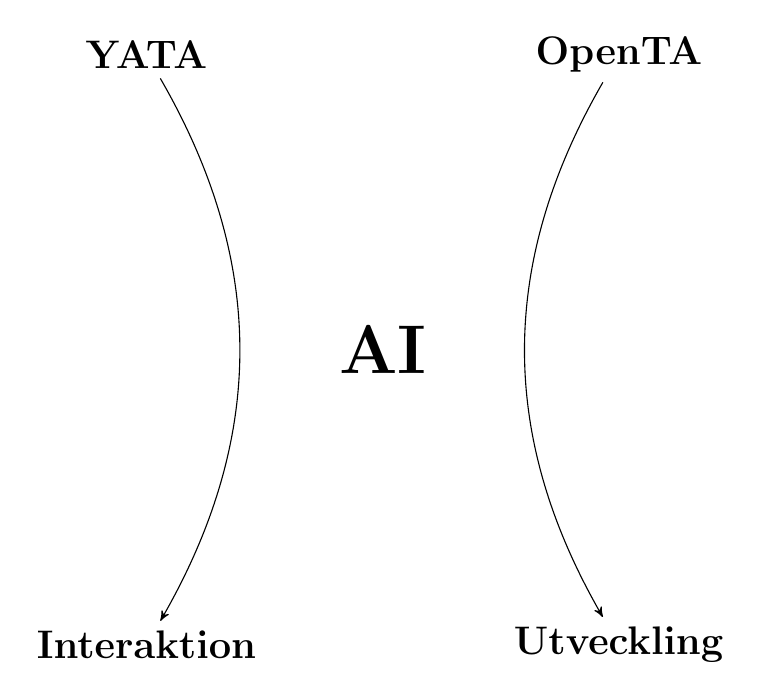
\begin{tikzpicture}[x=6cm, y=2.5cm, ->,>=stealth',auto, thick] 
% Column 1
\node [data part/.try] (yata) at (0,1.5) {\Large\textbf{YATA}};
\node [data part/.try] (openta) at (1,1.5) {\Large\textbf{OpenTA}};

\node [ai part/.try, minimum width=8cm] (ai) at (0.5, 0) {\Huge\textbf{AI}};

\node [results part/.try] (aitest) at (0,-1.5) {\Large\textbf{Interaktion}};
\node [data part/.try] (poss) at (1,-1.5) {\Large\textbf{Utveckling}};


% Connect them 
\begin{pgfonlayer}{background}[line width=1mm]
\path[main line/.try]
    (yata) edge[bend left] node [right] {} (aitest)
    (openta) edge[bend right] node [right] {} (poss);
\end{pgfonlayer}

\end{tikzpicture}
\end{document}